%%%%%%%%%%%%%%%%%%%%%%%%%%%%%%%%%%%%%%%%%%%%%%%%%%%%%%%%%%%%%%%%%%%%%%%%%%%%%%%%%%%%%%%%%%%%%%%%%%%%%%%
% Manuel d'Installation
% Bitume Legends Project
% CarrEniX
% Juin 2022
%%%%%%%%%%%%%%%%%%%%%%%%%%%%%%%%%%%%%%%%%%%%%%%%%%%%%%%%%%%%%%%%%%%%%%%%%%%%%%%%%%%%%%%%%%%%%%%%%%%%%%%

\documentclass[a4paper,12pt]{article}

\usepackage[utf8]{inputenc}
\usepackage[french]{babel}
\usepackage{geometry}
\usepackage{lipsum}
\usepackage{mathtools}
\usepackage[T1]{fontenc}
\usepackage{url}
\usepackage{longtable}
\usepackage[aboveskip=.5cm]{caption}
\usepackage{pdflscape}
\usepackage{xcolor}
\usepackage{fancyhdr}
\usepackage{graphicx,color}
\graphicspath{{../Medias}}

\newcommand{\hsp}{\hspace{20pt}}
\newcommand{\HRule}{\rule{\linewidth}{0.5mm}}
\newcommand{\btmlgs}{\textsl{Bitume Legends}}
\newcommand{\AI}{Intelligence Artificielle}
\newcommand{\FL}{\textsl{FL Studio 20}}
\newcommand{\CEX}{\textsc{CarrEniX}}
\newcommand{\SITE}{\(\mathtt{btms.games}\)}
\newcommand{\report}{Manuel d'Installation}
\renewcommand{\listfigurename}{Table des Annexes}
\renewcommand{\contentsname}{Table des Matières}
\newcommand\ytl[2]{\parbox[b]{10em}{\hfill{\color{cyan}\bfseries\sffamily 
    #1}~$\cdots\cdots$~}\makebox[0pt][c]{$\bullet$}\vrule\quad 
    \parbox[c]{5cm}{\vspace{7pt}\color{red!40!black!80}\raggedright\sffamily #2\\[7pt]}\\[-3pt]}

\pagestyle{fancy}
\lhead{\report}
\rhead{{\CEX}\\{\btmlgs}}   

\begin{document}
    % Homepage
    \begin{titlepage}
        \begin{center}
            
\includegraphics[scale=0.7]{logo192.png}\\[0.5cm]
            \textsc{\Large \report}\\[1.5cm]

            \HRule \\[0.4cm]
            { \LARGE \bfseries \btmlgs \\[0.4cm] }

            \HRule \\[2cm]
        
            \textsc{by \Large \CEX}\\[1.5cm]
        \end{center}
        \tableofcontents
        \begin{center}
            \HRule\\
            Lien pour télécharger le jeu: \url{https://btms.games/telechargement.html}
        \end{center}
    \end{titlepage}

    \section*{Introduction}
        Ce document est un manuel d'installation de \btmlgs.
        Pour installer \btmlgs, se référer à la partie concernant votre système d'exploitation.
        En cas de problèmes avec l'installation, 

    \section{Installation sur Windows}
        \begin{enumerate}
            \item
                \textbf{Télécharger} le fichier \texttt{btms$\_$windows.exe}
                depuis le site \\\url{https://btms.games/telechargement.html} en
                cliquant sur \\\fbox{\texttt{Téléchargement Windows 10+}}.\\
                \begin{figure}[h]
                    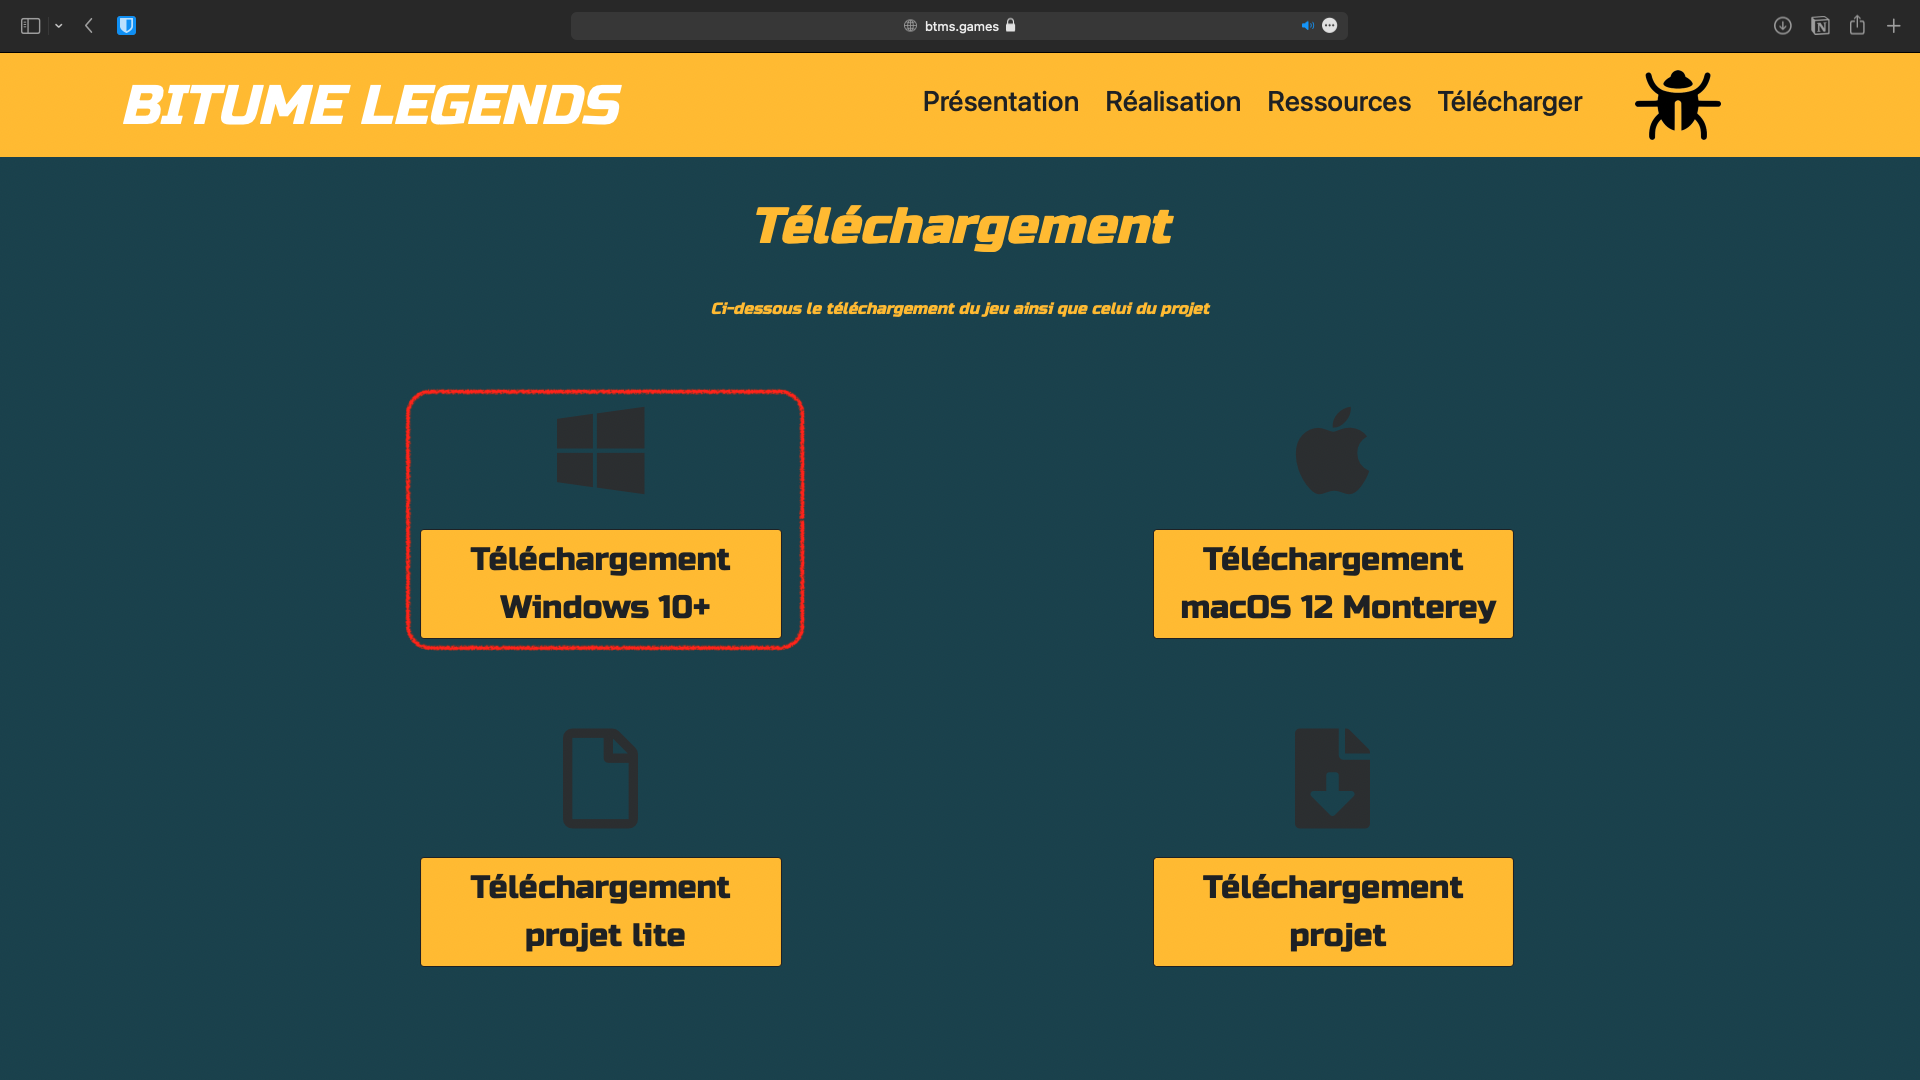
\includegraphics[scale=0.22]{dl_page_win.png}
                    \caption{Page de téléchargement}
                \end{figure}
            \item
                \textbf{Lancer} le fichier \texttt{btms$\_$windows.exe}.
            \clearpage
            \item 
                \textbf{Choisir} la langue de l'installateur puis cliquer sur
                \fbox{\texttt{Suivant}}.
                \begin{figure}[h]
                    \centering
                    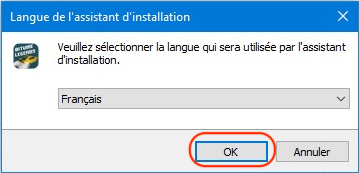
\includegraphics[scale=0.7]{langues.png}
                    \caption{Installateur - Langue}
                \end{figure}
            \item 
                \textbf{Choisir} le lieu d'installation, nous conseillons
                \\\texttt{C:$\backslash${Program} Files (x86)$\backslash${Bitume Legends}}
                puis cliquer sur \fbox{\texttt{Suivant}}.
                \begin{figure}[h]
                    \centering
                    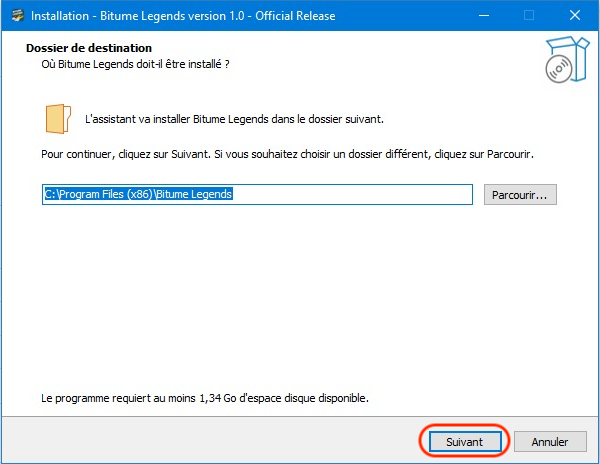
\includegraphics[scale=0.5]{install_location.png}
                    \caption{Installateur - Emplacement}
                \end{figure}
            \clearpage
            \item 
                \textbf{Cliquer} sur \texttt{Ajouter une icône sur le bureau}
                pour retrouver facilement \btmlgs puis cliquer sur \fbox{\texttt{Suivant}}.
                \begin{figure}[h]
                    \centering
                    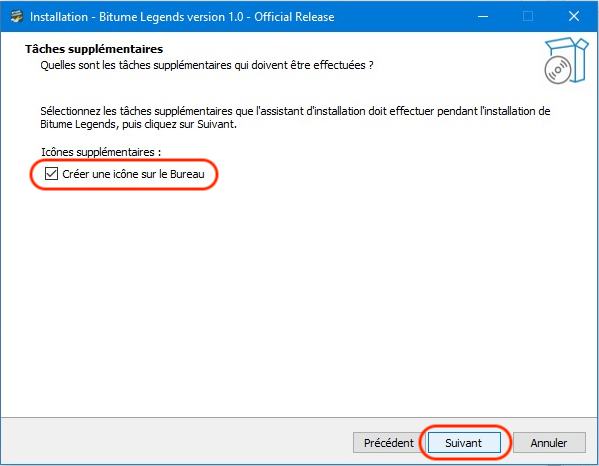
\includegraphics[scale=0.4]{shortcut.png}
                    \caption{Installateur - Icône}
                \end{figure}
            \item
                \textbf{Vérifier} l'installation et cliquer sur \fbox{\texttt{Installer}}.
                \begin{figure}[h]
                    \centering
                    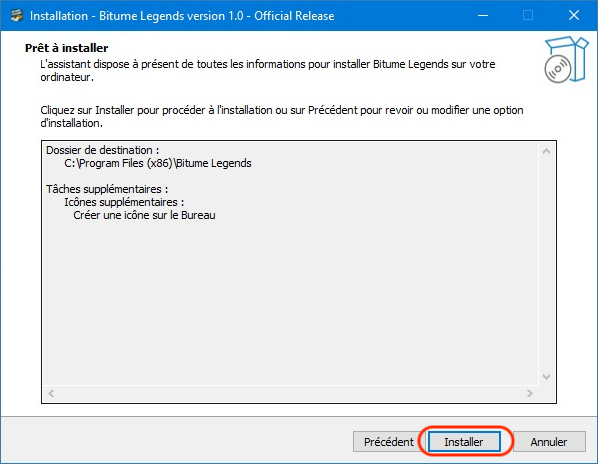
\includegraphics[scale=0.4]{recap.png}
                    \caption{Installateur - Récapitulatif}
                \end{figure}
            \clearpage
            \item 
                \textbf{Attendre} que le programme s'installe et cliquer sur
                \fbox{\texttt{Terminer}}.
                \begin{figure}[h]
                    \centering
                    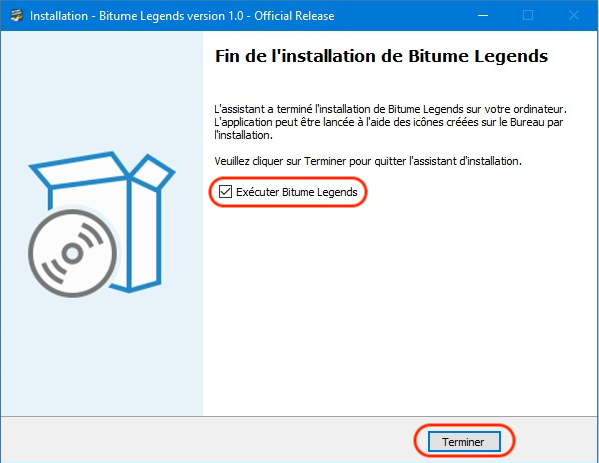
\includegraphics[scale=0.5]{end_process.png}
                    \caption{Installateur - Fin}
                \end{figure}
            \item 
                \textbf{Revenir} sur le bureau.
            \item
                \textbf{Cliquer} sur \fbox{\btmlgs} pour ouvrir le jeu.
        \end{enumerate}
        \clearpage

    \section{Installation sur macOS}
        \begin{enumerate}
            \item
                \textbf{Télécharger} le fichier \texttt{btms$\_$macos.dmg.zip}
                depuis le site \\\url{https://btms.games/telechargement.html} en
                cliquant sur \\\fbox{\texttt{Téléchargement macOS 12 Monterey}}.\\
                \begin{figure}[h]
                    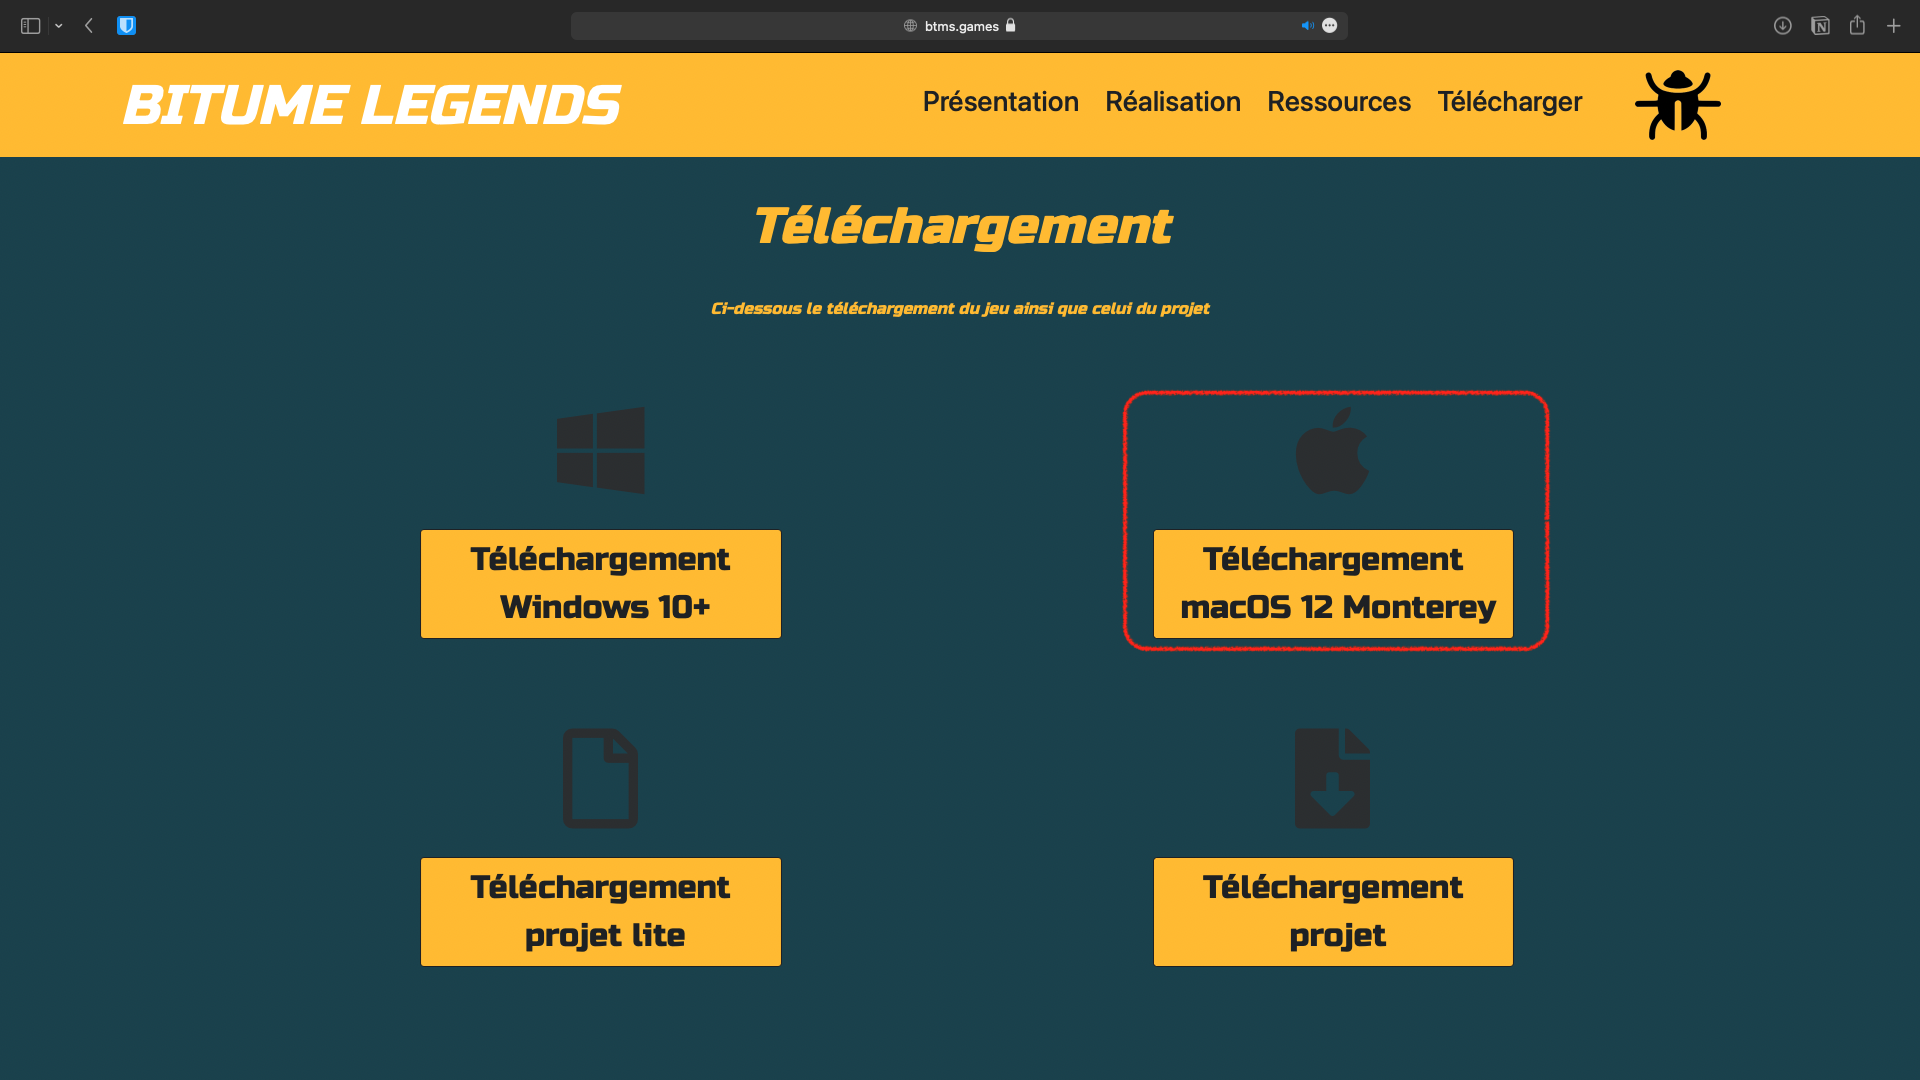
\includegraphics[scale=0.22]{dl_page_mac.png}
                    \caption{Page de téléchargement}
                \end{figure}
            
            \clearpage
            \item
                \textbf{Décompresser} le fichier \texttt{btms$\_$macos.dmg.zip}
                \footnote{Parfois, l'installateur est déjà décompressé. Si c'est
                le cas, merci de passer au point suivant.}.\\
                \begin{figure}[h]
                    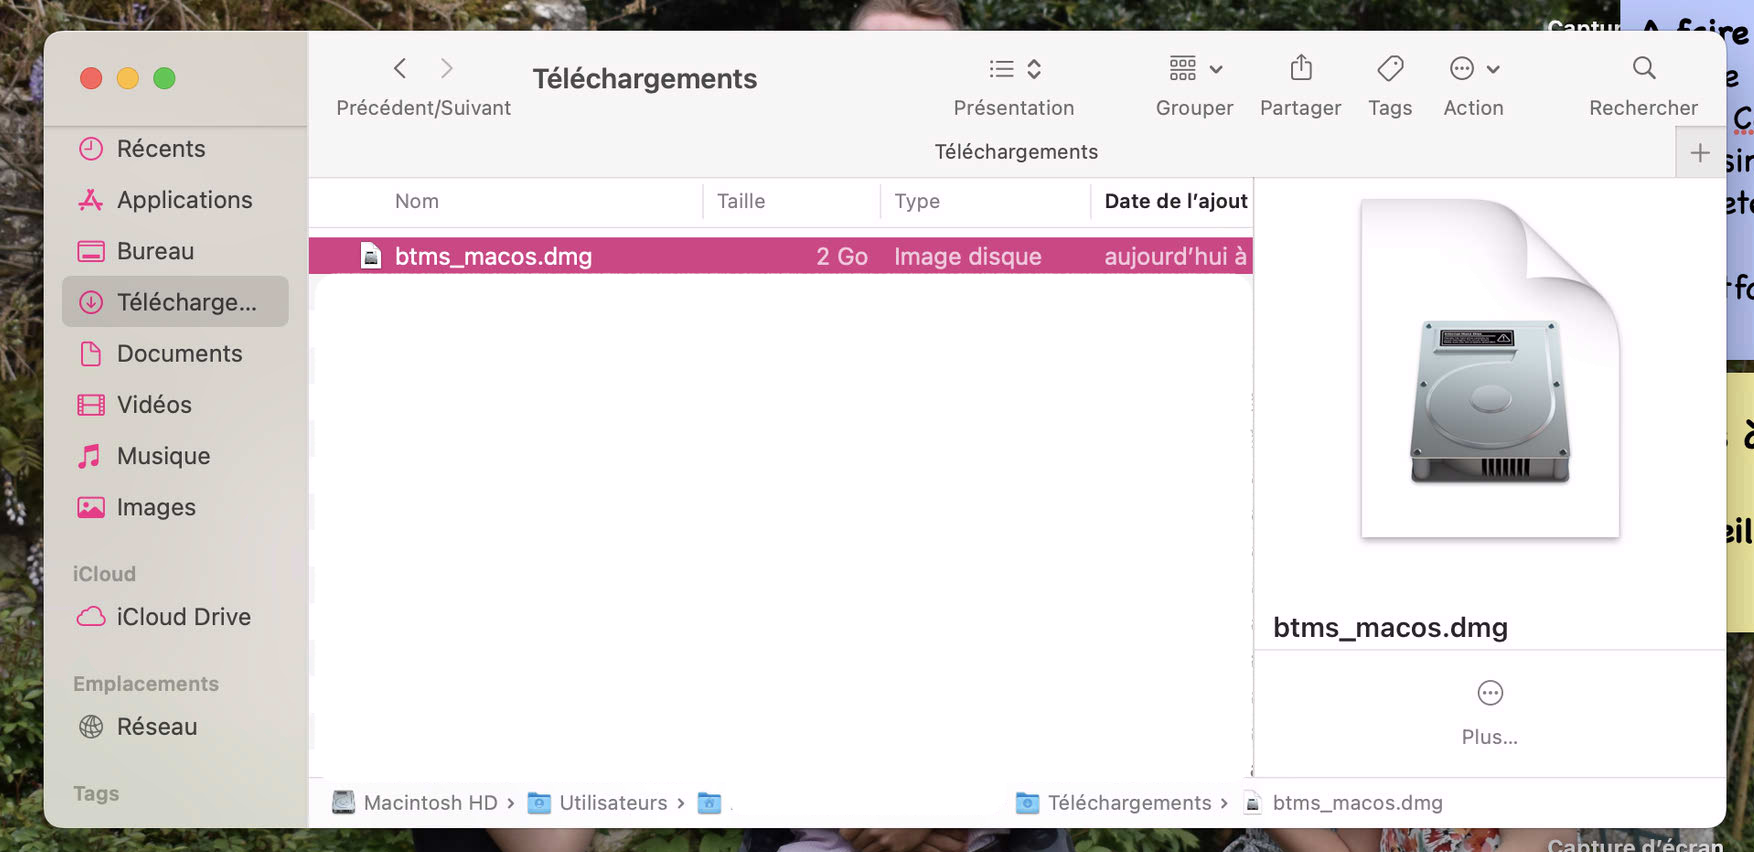
\includegraphics[scale=0.5]{dmg_in_dl.png}
                    \caption{Dossier Téléchargement}
                \end{figure}
            \item
                \textbf{Lancer} le fichier \texttt{btms$\_$macos.dmg}.
            \item
                \textbf{Ouvrir} \fbox{\textsl{Bitume Legends}} depuis le bureau.
            
            \clearpage
            \item
                \textbf{Déposer} l'application \fbox{\btmlgs} dans le dossier
                \texttt{Applications}.\\
                \begin{figure}[h]
                    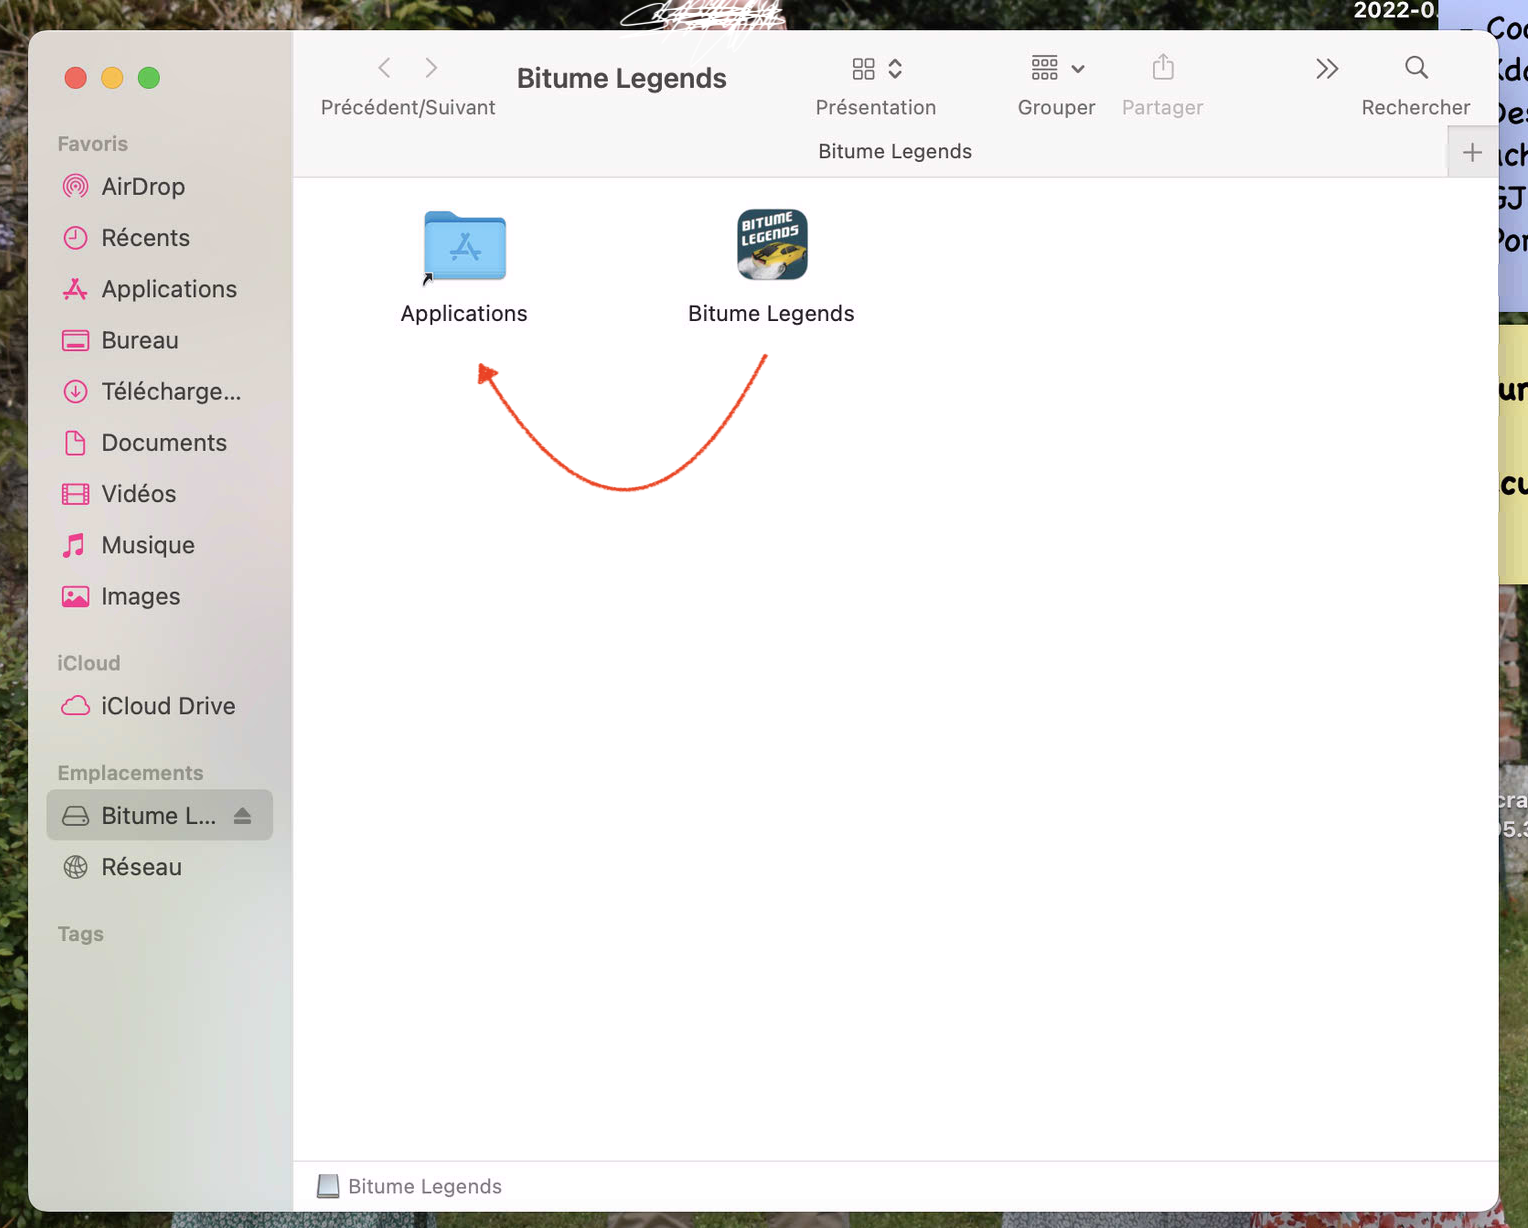
\includegraphics[scale=0.55]{in_btms-dmg.png}
                    \caption{btms$\_$macos.dmg}
                \end{figure}
            \item
                \textbf{Fermer} l'installateur et l'éjecter.
            \item
                \textbf{Ouvrir} le \textsl{Launchpad} (Afficher les applications).
            \item
                \textbf{Lancer} l'application \fbox{\btmlgs}.
        \end{enumerate}
        \clearpage

    \section{Problèmes d'installation avec Windows}
        En temps qu'étudiants, et n'ayant pas une licence professionnelle, nous ne pouvons 
        pas faire vérifier notre jeu par \textsl{Microsoft}.
        Cela implique que l'application peut poser problème à l'installation.
        Pour cela, nous avons prévu une solution pour forcer l'installation.
        Si la fenêtre suivante apparaît, merci de suivre la procédure ci-dessous.
        \begin{figure}[h]
            \centering
            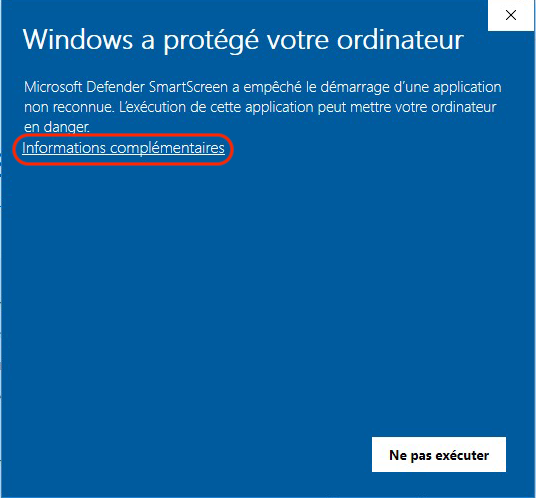
\includegraphics[scale=0.7]{error_win.png}
            \caption{Erreur d'installation}
        \end{figure}
        \begin{itemize}
            \item
                \textbf{Cliquer} sur \fbox{\texttt{Informations Complémentaires}}.
            \clearpage
            \item
                \textbf{Cliquer} sur \fbox{\texttt{Exécuter quand même}}.
                \begin{figure}[h]
                    \centering
                    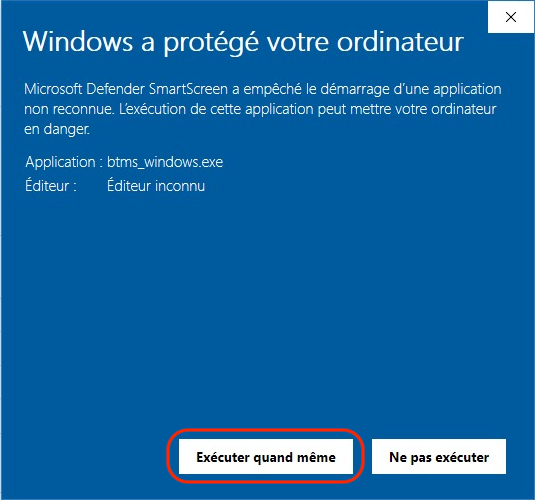
\includegraphics[scale=0.7]{exec_qdmm.png}
                    \caption{Exécuter quand même}
                \end{figure}
            \item
                \textbf{S'identifier} si besoin.
            \item
                \textbf{Revenir} à l'étape numéro 3.
        \end{itemize}


    \clearpage
    \section{Problèmes d'installation avec macOS}
        En temps qu'étudiants, et n'ayant pas une licence professionnelle, nous ne pouvons 
        pas faire vérifier notre jeu par \textsl{Apple}.
        Cela implique que l'application peut poser problème à l'installation.
        Pour cela, nous avons prévu une solution pour forcer l'installation.
        Si la fenêtre suivante apparaît, merci de suivre la procédure ci-dessous.
        \begin{figure}[h]
            \centering
            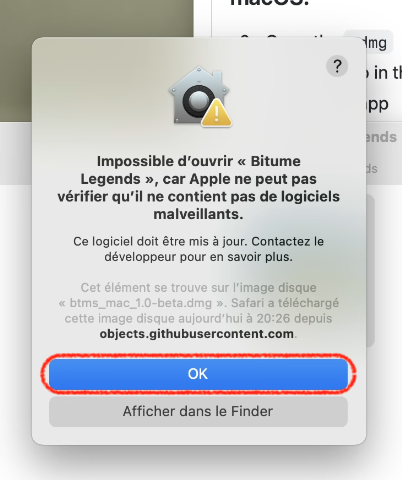
\includegraphics[scale=0.8]{install_mac_error.png}
            \caption{Erreur d'installation}
        \end{figure}
    
        \begin{itemize}
            \item
                \textbf{Cliquer} sur \fbox{\texttt{OK}} pour fermer la pop-up.
            \item
                \textbf{Ouvrir} l'application \textsl{Préférences Système}.
            
            \clearpage
            \item
                \textbf{Cliquer} sur l'icône \fbox{\texttt{Sécurité et Confidentialité}}.
                \begin{figure}[h]
                    \centering
                    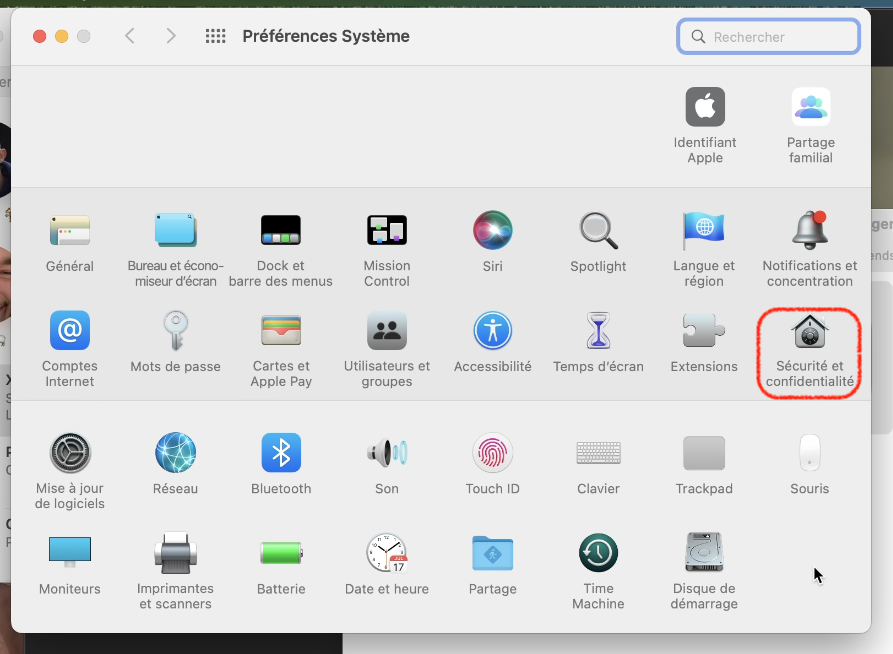
\includegraphics[scale=0.5]{install_macos_sp.png}
                    \caption{Préférences Système}
                \end{figure}

            \clearpage
            \item
                \textbf{Cliquer} sur \fbox{\texttt{Ouvrir quand même}}\; dans l'onglet
                \fbox{\texttt{Général}}.
                \begin{figure}[h]
                    \centering
                    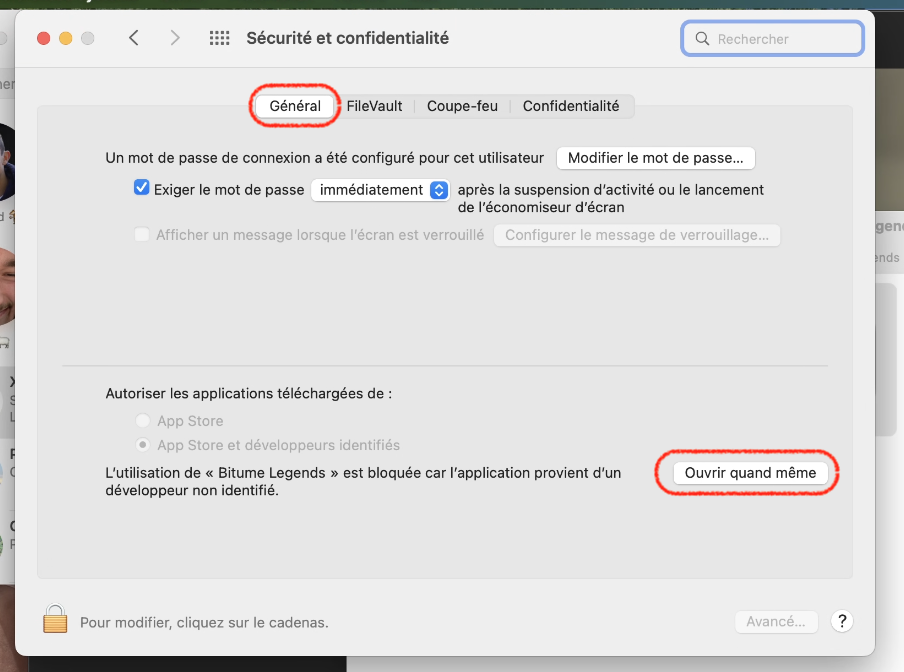
\includegraphics[scale=0.5]{install_macos_security.png}
                    \caption{Sécurité et Confidentialité}
                \end{figure}

            \clearpage
            \item
                \textbf{Valider} l'ouverture du jeu sur la pop-up.\\
                \begin{figure}[h]
                    \centering
                    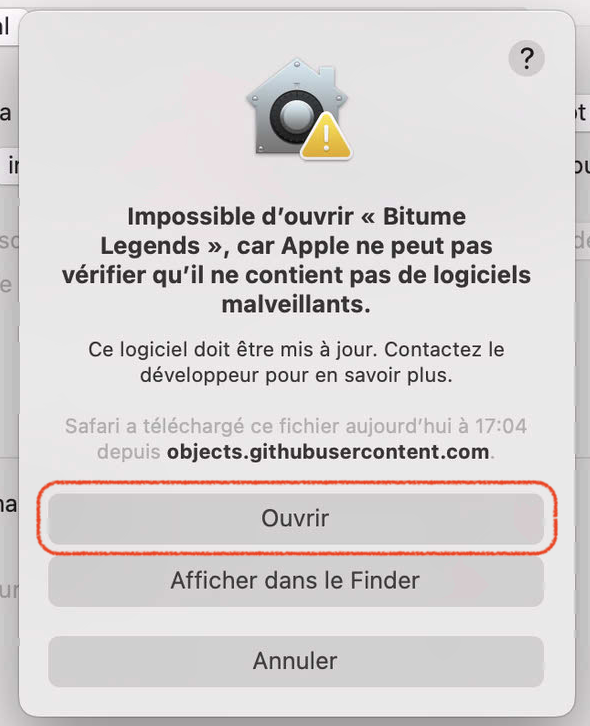
\includegraphics[scale=1]{ok_mac.png}
                    \caption{Autorisation}
                \end{figure}
        \end{itemize}

    \clearpage
    \section{Procédure de Désinstallation}
        \subsection*{Windows}
            \begin{itemize}
                \item
                    \textbf{Aller} à l'endroit où le jeu est installé.
                \item
                    \textbf{Cliquer} sur \fbox{\texttt{uninstall.exe}}.
                \item
                    \textbf{Suivre} les étapes indiquées.
            \end{itemize}
        \subsection*{macOS}
            Pour désinstaller \btmlgs\;sur \textsl{macOS}, veuillez suivre la procédure habituelle.

\end{document}
